% ថ្នាក់ទី ១១ (វិទ្យាសាស្ត្រ) · ជំពូកទី ៥ · មេរៀនទី ៤ · សៀវភៅភាគ ២ ទំព័រ ៥៤–៧៦
\chapter{អនុវត្តន៍ដេរីវេចំពោះសមីការនិងវិសមីការ}

\begin{objBox}[វត្ថុបំណង]
\begin{enumerate}[1]
  \item សិក្សាទៅតាមតម្លៃប៉ារ៉ាម៉ែត្រពីអត្ថិភាពឫស ទីតាំងឫសធៀបនឹងចំនួន និងចំនួនឫសនៃសមីការដឺក្រេទី $3$ និងសមីការដឺក្រេទី $4$ ដោយប្រើក្រាប
  \item ដោះស្រាយវិសមីការដឺក្រេទី $3$ និងវិសមីការដឺក្រេទី $4$ ដោយប្រើដេរីវេនិងក្រាប
  \item បង្ហាញវិសមីការដឺក្រេទី $3$ និងវិសមីការដឺក្រេទី $4$ ដោយប្រើដេរីវេនិងក្រាប ។
\end{enumerate}
\end{objBox}

\section{ការអនុវត្តដេរីវេចំពោះសមីការ}

ដោយប្រើក្រាបនៃអនុគមន៍ $y = f(x)$ គេអាចបញ្ជាក់បានដោយងាយពីអត្ថិភាពឫស ទីតាំងឫសធៀបនឹងចំនួន និងចំនួនឫសនៃសមីការ $f(x) = \lambda$ ទៅតាមតម្លៃប៉ារ៉ាម៉ែត្រ $\lambda$ ។

\subsection{ការអនុវត្តដេរីវេចំពោះសមីការដឺក្រេទី 3}

\begin{example}[ឧទាហរណ៍]
អនុគមន៍ $y = f(x) = x^3 + 3x^2 - 2$ មានក្រាប $C$ ។
\begin{enumerate}[a]
  \item សង់ក្រាប $C$ នៃអនុគមន៍ $f$ ។
  \item សិក្សាដោយប្រើក្រាបហ្វិកទៅតាមតម្លៃប៉ារ៉ាម៉ែត្រ $\lambda$ អត្ថិភាពនិងចំនួនឫសនៃសមីការ $x^3 + 3x^2 - 2 = \lambda$ ។
\end{enumerate}
\end{example}
\ans
\begin{enumerate}[a]
  \item សង់ក្រាបនៃ $f$ ៖ ដែនកំណត់ $D = \mathbb{R}$ ។ ដេរីវេ $f'(x) = 3x^2 + 6x = 3x(x + 2)$ ។ បើ $f'(x) = 0$ នោះ $x = 0$ ឬ $x = -2$ ។ ចំពោះ $x = 0$ គេបាន $f(0) = -2$ និងចំពោះ $x = -2$ គេបាន $f(-2) = 2$ ។ លីមីតចុងដែនកំណត់ ៖ $\displaystyle\lim_{x \to -\infty} f(x) = \lim_{x \to -\infty} x^3\left(1 + \frac{3}{x} - \frac{2}{x^3}\right) = -\infty$ និង $\displaystyle\lim_{x \to +\infty} f(x) = +\infty$ ។
  \begin{center}
  \begin{tikzpicture}
    \tkzTabInit[lgt=1.6,espcl=2]{$x$ /0.8, $f'(x)$ /0.8, $f(x)$ /1.6}{$-\infty$, $-2$, $0$, $+\infty$}
    \tkzTabLine{, +, z, -, z, +, }
    \tkzTabVar{-/$-\infty$, +/$2$, -/$-2$, +/$+\infty$}
  \end{tikzpicture}
  \end{center}
  ក្រាបប្រសព្វអ័ក្ស $y'oy$ $\Rightarrow x = 0$, $y = -2$ ។ ក្រាបប្រសព្វអ័ក្ស $x'ox$ $\Rightarrow y = 0$ ៖
  \[ \begin{aligned} x^3 + 3x^2 - 2 = 0 &\Leftrightarrow x^2(x + 1) + 2(x^2 - 1) = 0\\ &\Leftrightarrow (x + 1)(x^2 + 2x - 2) = 0 \end{aligned} \]
  នាំឱ្យ $x = -1$ ឬ $(x + 1)^2 = 3$ គឺ $x = -1 \pm\sqrt{3}$ ។
  \begin{center}
  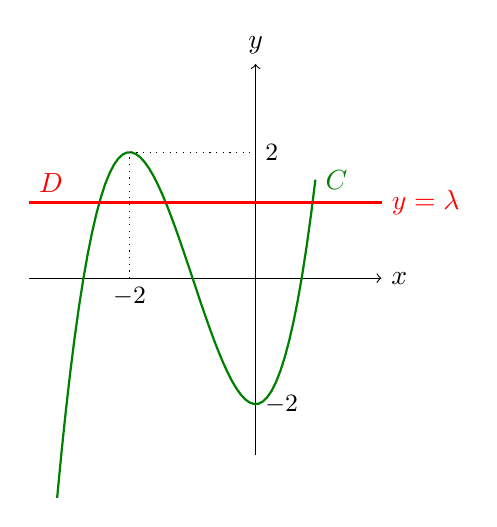
\begin{tikzpicture}[scale=0.8]
    \draw[->] (-3.6,0) -- (2,0) node[right] {$x$};
    \draw[->] (0,-2.8) -- (0,3.4) node[above] {$y$};
    \draw[thick,green!50!black,domain=-3.15:0.95,samples=60] plot (\x,{(\x)^3+3*(\x)^2-2}) node[right] {$C$};
    \draw[thick,red] (-3.6,1.2) node[above right] {$D$} -- (2,1.2) node[right] {$y = \lambda$};
    \draw[dotted] (-2,0) -- (-2,2) -- (0,2) node[right] {\small $2$};
    \node[right] at (0,-2) {\small $-2$}; \node[below] at (-2,0) {\small $-2$};
  \end{tikzpicture}
  \end{center}
  \item សិក្សាទៅតាមតម្លៃ $\lambda$ អត្ថិភាពនិងចំនួនឫសនៃសមីការ ។ គេបាន $x^3 + 3x^2 - 2 = \lambda$ $(1)$ ជាសមីការអាប់ស៊ីសនៃចំណុចប្រសព្វរវាងក្រាប $C$ និងបន្ទាត់ $D : y = \lambda$ ។ សង់បន្ទាត់ $D$ នៅក្នុងតម្រុយតែមួយ ហើយនៅត្រង់ផ្នែកណាមួយដែលជួបក្រាប $C$ បានច្រើនចំណុចបំផុត ។ ចំនួនឫសនៃសមីការ ស្មើនឹងចំនួនចំណុចប្រសព្វរវាង $C$ និង $D$ ។
  \begin{itemize}
    \item បើ $\lambda > 2$ នោះសមីការ $(1)$ មានឫសតែ $1$ គត់ ។
    \item បើ $\lambda = 2$ នោះសមីការ $(1)$ មានឫសឌុបនិងឫសមួយផ្សេងទៀត ។
    \item បើ $-2 < \lambda < 2$ នោះសមីការ $(1)$ មានឫស $3$ ផ្សេងគ្នា ។
    \item បើ $\lambda = -2$ នោះសមីការ $(1)$ មានឫសឌុបនិងឫសមួយផ្សេងទៀត ។
    \item បើ $\lambda < -2$ នោះសមីការ $(1)$ មានឫសតែ $1$ គត់ ។
  \end{itemize}
\end{enumerate}

\begin{example}[លំហាត់គំរូ]
សិក្សាដោយប្រើក្រាបហ្វិកទៅតាមតម្លៃ $m$ អត្ថិភាពនិងទីតាំងឫសនៃសមីការ $x^3 - 3x - m = 0$ ធៀបនឹងចំនួន $0$ និង $1$ ។
\end{example}
\ans
ជំហានទី $1$ ៖ សង់ក្រាបនៃអនុគមន៍ $y = x^3 - 3x$ ។ គេបាន $y' = 3x^2 - 3$ ។ បើ $y' = 0$, $3x^2 - 3 = 0 \Leftrightarrow x^2 = 1 \Rightarrow x = \pm 1$ ។ ចំពោះ $x = -1$ គេបាន $y = 2$ និងចំពោះ $x = 1$ គេបាន $y = -2$ ។ $\displaystyle\lim_{x \to +\infty}(x^3 - 3x) = +\infty$, $\displaystyle\lim_{x \to -\infty}(x^3 - 3x) = -\infty$ ។
\begin{center}
\begin{tikzpicture}
  \tkzTabInit[lgt=1.6,espcl=2]{$x$ /0.8, $y'$ /0.8, $y$ /1.6}{$-\infty$, $-1$, $1$, $+\infty$}
  \tkzTabLine{, +, z, -, z, +, }
  \tkzTabVar{-/$-\infty$, +/$2$, -/$-2$, +/$+\infty$}
\end{tikzpicture}
\end{center}
ក្រាបប្រសព្វអ័ក្ស $(x'ox) \Rightarrow y = 0$ ៖ $x^3 - 3x = 0 \Leftrightarrow x(x^2 - 3) = 0 \Leftrightarrow x = 0$ ឬ $x = \pm\sqrt{3}$ ។

ជំហានទី $2$ ៖ បំប្លែងសមីការឱ្យមានរាង $f(x) = m$ ៖ $x^3 - 3x = m$ ។

ជំហានទី $3$ ៖ សង់បន្ទាត់ដេកមានសមីការ $y = m$ នៅក្នុងតម្រុយតែមួយហើយនៅត្រង់ផ្នែកណាដែលបន្ទាត់ជួបក្រាបបានច្រើនចំណុចបំផុត ។

\begin{center}
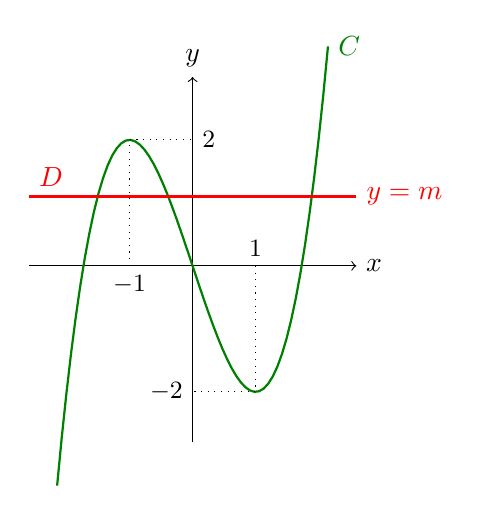
\begin{tikzpicture}[scale=0.8]
  \draw[->] (-2.6,0) -- (2.6,0) node[right] {$x$};
  \draw[->] (0,-2.8) -- (0,3) node[above] {$y$};
  \draw[thick,green!50!black,domain=-2.15:2.15,samples=60] plot (\x,{(\x)^3-3*\x}) node[right] {$C$};
  \draw[thick,red] (-2.6,1.1) node[above right] {$D$} -- (2.6,1.1) node[right] {$y = m$};
  \draw[dotted] (-1,0) -- (-1,2) -- (0,2) node[right] {\small $2$};
  \draw[dotted] (1,0) -- (1,-2) -- (0,-2) node[left] {\small $-2$};
  \node[below] at (-1,0) {\small $-1$}; \node[above] at (1,0) {\small $1$};
\end{tikzpicture}
\end{center}

ជំហានទី $4$ ៖ ប្រើក្រាបដើម្បីសិក្សាទៅតាមតម្លៃ $m$ នូវអត្ថិភាពនិងទីតាំងឫសធៀបនឹងចំនួន $0$ និង $1$ ។ សន្មត $x_1, x_2, x_3$ ជាឫសនៃសមីការដែល $x_1 \le x_2 \le x_3$ ។
\begin{itemize}
  \item បើ $m > 2$ នោះសមីការមានឫសតែមួយគត់ $x_3$ ដែល $0 < 1 < x_3$ ។
  \item បើ $m = 2$ នោះសមីការមានឫសដែល $x_1 = x_2 = -1 < 0 < 1 < x_3$ ។
  \item បើ $0 < m < 2$ នោះសមីការមានឫសបីផ្សេងគ្នាដែល $x_1 < x_2 < 0 < 1 < x_3$ ។
  \item បើ $m = 0$ នោះសមីការមានឫសបីផ្សេងគ្នាដែល $x_1 < x_2 = 0 < 1 < x_3$ ។
  \item បើ $-2 < m < 0$ នោះសមីការមានឫសបីផ្សេងគ្នាដែល $x_1 < 0 < x_2 < 1 < x_3$ ។
  \item បើ $m = -2$ នោះសមីការមានឫសដែល $x_1 < 0 < 1 = x_2 = x_3$ ។
  \item បើ $m < -2$ នោះសមីការមានឫសតែមួយគត់ដែល $x_1 < 0 < 1$ ។
\end{itemize}

\begin{formulaBox}[ជាទូទៅ]
សមីការ $ax^3 + bx^2 + cx + d = \lambda$ មានឫសជាអាប់ស៊ីសនៃចំណុចប្រសព្វរវាងក្រាបនៃ $y = ax^3 + bx^2 + cx + d$ និងបន្ទាត់មានសមីការ $y = \lambda$ ។
\end{formulaBox}

\begin{pro}
អនុគមន៍ $y = x^3 - 3x + 2$ មានក្រាប $C$ ។ រកតម្លៃ $a$ ដើម្បីឱ្យសមីការ $x^3 - 3x + 2 = a$ ៖ \quad ក. មានឫសបីផ្សេងគ្នា ។ \quad ខ. មានឫសវិជ្ជមានពីរផ្សេងគ្នា និងឫសអវិជ្ជមានមួយទៀត ។
\ans
ក. $0 < a < 4$ \quad ខ. $0 < a < 2$ ។
\end{pro}

\subsection{ការអនុវត្តដេរីវេចំពោះសមីការប៊ីការេ}

\begin{example}[ឧទាហរណ៍]
អនុគមន៍ $y = x^4 - 2x^2$ មានក្រាប $C$ ។
\begin{enumerate}[a]
  \item សង់ក្រាប $C$ នៃអនុគមន៍ ។
  \item ដោយប្រើក្រាប $(C)$ សិក្សាទៅតាមតម្លៃ $m$ អត្ថិភាពនិងចំនួនឫសនៃសមីការ $x^4 - 2x^2 - m = 0$ ។
\end{enumerate}
\end{example}
\ans
\begin{enumerate}[a]
  \item $y' = 4x^3 - 4x = 4x(x^2 - 1)$ ។ $y' = 0 \Leftrightarrow x = 0$ ឬ $x = \pm 1$ ។ ចំពោះ $x = 0$, $y = 0$ និងចំពោះ $x = \pm 1$, $y = -1$ ។ $\displaystyle\lim_{x \to \pm\infty}(x^4 - 2x^2) = \lim_{x \to \pm\infty} x^4\left(1 - \frac{2}{x^2}\right) = +\infty$ ។
  \begin{center}
  \begin{tikzpicture}
    \tkzTabInit[lgt=1.6,espcl=1.8]{$x$ /0.8, $y'$ /0.8, $y$ /1.6}{$-\infty$, $-1$, $0$, $1$, $+\infty$}
    \tkzTabLine{, -, z, +, z, -, z, +, }
    \tkzTabVar{+/$+\infty$, -/$-1$, +/$0$, -/$-1$, +/$+\infty$}
  \end{tikzpicture}
  \end{center}
  បើ $x = 0$ នាំឱ្យ $y = 0$ ។ បើ $y = 0$, $x^2(x^2 - 2) = 0$ នាំឱ្យ $x = 0$ ឬ $x = \pm\sqrt{2}$ ។
  \item សមីការ $x^4 - 2x^2 = m$ ៖
  \begin{itemize}
    \item បើ $m > 0$ នោះសមីការមានឫស $2$ ផ្សេងគ្នា ។
    \item បើ $m = 0$ នោះសមីការមានឫស $4$ គឺ $0$ ជាឫសឌុប និងឫសពីរផ្សេងទៀតត្រង់ $x = \pm\sqrt{2}$ ។
    \item បើ $-1 < m < 0$ នោះសមីការមានឫស $4$ ផ្សេងគ្នា ។
    \item បើ $m = -1$ នោះសមីការមានឫសឌុប $2$ ត្រង់ $x = \pm 1$ ។
    \item បើ $m < -1$ នោះសមីការគ្មានឫស ។
  \end{itemize}
\end{enumerate}

\begin{center}
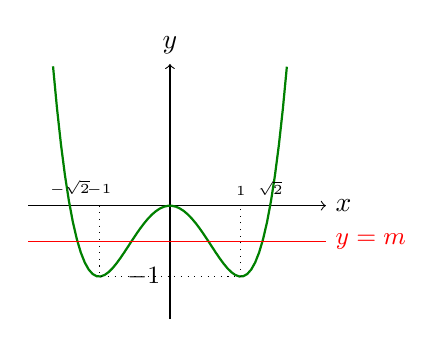
\begin{tikzpicture}[scale=0.9]
  \draw[->] (-2,0) -- (2.2,0) node[right] {$x$};
  \draw[->] (0,-1.6) -- (0,2) node[above] {$y$};
  \draw[thick,green!50!black,domain=-1.65:1.65,samples=60] plot (\x,{(\x)^4-2*(\x)^2});
  \draw[red] (-2,-0.5) -- (2.2,-0.5) node[right] {\small $y = m$};
  \draw[dotted] (-1,0) -- (-1,-1) -- (1,-1) -- (1,0);
  \foreach \x/\l in {-1.414/-\sqrt{2},-1/-1,1/1,1.414/\sqrt{2}} \node[above] at (\x,0) {\tiny $\l$};
  \node[left] at (0,-1) {\small $-1$};
\end{tikzpicture}
\end{center}

\begin{example}[លំហាត់គំរូ]
គេឱ្យអនុគមន៍ $f(x) = x^4 - 2x^2 + 2$ និងក្រាប $C$ ។ សិក្សាទៅតាមតម្លៃប៉ារ៉ាម៉ែត្រ $\lambda$ អត្ថិភាពនិងទីតាំងឫសនៃសមីការ $x^4 - 2x^2 + 2 = \lambda$ ធៀបនឹងចំនួន $-1$ និង $1$ តាមក្រាប ។
\end{example}
\ans
ជំហានទី $1$ ៖ សមីការមានរាង $x^4 - 2x^2 + 2 = \lambda$ ។ អនុគមន៍ $f$ មានអប្បបរមា $f(\pm 1) = 1$ និងអតិបរមាធៀប $f(0) = 2$ ។

ជំហានទី $2$ ៖ សង់បន្ទាត់ដេកមានសមីការ $y = \lambda$ ។

\begin{center}
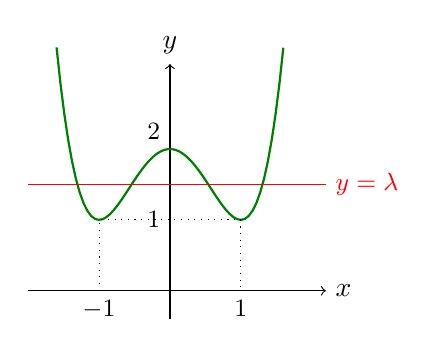
\begin{tikzpicture}[scale=0.9]
  \draw[->] (-2,0) -- (2.2,0) node[right] {$x$};
  \draw[->] (0,-0.4) -- (0,3.2) node[above] {$y$};
  \draw[thick,green!50!black,domain=-1.6:1.6,samples=60] plot (\x,{(\x)^4-2*(\x)^2+2});
  \draw[red] (-2,1.5) -- (2.2,1.5) node[right] {\small $y = \lambda$};
  \draw[dotted] (-1,0) -- (-1,1) -- (1,1) -- (1,0);
  \node[below] at (-1,0) {\small $-1$}; \node[below] at (1,0) {\small $1$};
  \node[above left] at (0,2) {\small $2$}; \node[left] at (0,1) {\small $1$};
\end{tikzpicture}
\end{center}

ជំហានទី $3$ ៖ សន្មត $x_1, x_2, x_3$ និង $x_4$ ជាឫសនៃសមីការដែល $x_1 \le x_2 \le x_3 \le x_4$ ។ សិក្សាដោយប្រើក្រាបទៅតាមតម្លៃ $\lambda$ ៖
\begin{itemize}
  \item បើ $\lambda > 2$ នោះសមីការមានឫសពីរផ្សេងគ្នាដែល $x_1 < -1 < 1 < x_2$ ។
  \item បើ $\lambda = 2$ នោះសមីការមានឫសបួនដែល $x_1 < -1 < x_2 = x_3 = 0 < 1 < x_4$ ។
  \item បើ $1 < \lambda < 2$ នោះសមីការមានឫសបួនផ្សេងគ្នាដែល $x_1 < -1 < x_2 < x_3 < 1 < x_4$ ។
  \item បើ $\lambda = 1$ នោះសមីការមានឫសបួនដែល $x_1 = x_2 = -1 < x_3 = x_4 = 1$ ។
  \item បើ $\lambda < 1$ នោះសមីការគ្មានឫសទេ ។
\end{itemize}

\begin{formulaBox}[ជាទូទៅ]
សមីការ $ax^4 + bx^2 + c = \lambda$ មានឫសជាអាប់ស៊ីសនៃចំណុចប្រសព្វរវាងក្រាបនៃ $y = ax^4 + bx^2 + c$ និងបន្ទាត់មានសមីការ $y = \lambda$ ។
\end{formulaBox}

\begin{pro}
គេឱ្យក្រាបនៃអនុគមន៍ $y = x^4 - 4x^2 + 3$ ។ រកតម្លៃ $m$ ដើម្បីឱ្យសមីការ $x^4 - 4x^2 = m - 3$ ៖ \quad ក. មានឫសបួនផ្សេងគ្នា ។ \quad ខ. មានឫសពីរផ្សេងគ្នានៅក្រៅចន្លោះ $[-2, 2]$ ។
\ans
ក. $-1 < m < 3$ \quad ខ. $m > 3$ ។
\end{pro}

\section{ការអនុវត្តដេរីវេចំពោះវិសមីការ}
\subsection{ការអនុវត្តដេរីវេចំពោះវិសមីការដឺក្រេទី 3}

\begin{example}[ឧទាហរណ៍]
បង្ហាញថាវិសមីការ $x^3 + x + 2 > 0$ ផ្ទៀងផ្ទាត់ចំពោះ $x > -1$ ។
\end{example}
\textbf{របៀបទី $1$} ៖ ប្រើប្រាស់អនុគមន៍ $y = x^3 + x + 2$ ។ $y' = 3x^2 + 1 > 0$ ចំពោះ $\forall x \in \mathbb{R}$ ។ $y'' = 6x$, បើ $y'' = 0$, $6x = 0 \Rightarrow x = 0$ ។ $\displaystyle\lim_{x \to +\infty}(x^3 + x + 2) = +\infty$, $\displaystyle\lim_{x \to -\infty}(x^3 + x + 2) = -\infty$ ។ បើ $x = 0$, $y = 2$ ។ បើ $y = 0$, $x^3 + x + 2 = 0$ សមមូល $(x + 1)(x^2 - x + 2) = 0$ ឬ $x = -1$ ព្រោះសមីការ $x^2 - x + 2 = 0$ គ្មានឫស ។ តាមក្រាបគ្រប់ចំណុច $(x, y)$ ដែលមាន $y > 0$ ត្រូវស្ថិតនៅផ្នែកខាងលើអ័ក្សអាប់ស៊ីស ហើយត្រូវគ្នានឹង $x > -1$ ។ ដូច្នេះ វិសមីការ $x^3 + x + 2 > 0$ ផ្ទៀងផ្ទាត់ចំពោះ $x > -1$ ។

\begin{center}
\begin{tikzpicture}[scale=0.7]
  \draw[->] (-2.2,0) -- (2.2,0) node[right] {$x$};
  \draw[->] (0,-2.5) -- (0,5.5) node[above] {$y$};
  \draw[thick,green!50!black,domain=-1.6:1.45,samples=60] plot (\x,{(\x)^3+\x+2}) node[right] {\small $x^3 + x + 2$};
  \node[below left] at (-1,0) {\small $-1$}; \node[above left] at (0,2) {\small $2$};
\end{tikzpicture}
\end{center}

\textbf{របៀបទី $2$} ៖ ប្រើទិសដៅអថេរភាពនៃអនុគមន៍ $y = x^3 + x + 2$ ។ គេបាន $y' = 3x^2 + 1 > 0$, $\forall x \in \mathbb{R}$ $\Rightarrow$ អនុគមន៍ $y$ ជាអនុគមន៍កើនលើ $\mathbb{R}$ ។ បើ $x > -1 \Rightarrow y(x) > y(-1)$ (លក្ខណៈអនុគមន៍កើន) ។ ដោយ $y(-1) = (-1)^3 + (-1) + 2 = 0$ $\Rightarrow y(x) > 0$ ។ ដូច្នេះ វិសមីការ $x^3 + x + 2 > 0$ ផ្ទៀងផ្ទាត់ចំពោះ $x > -1$ ។

\begin{example}[លំហាត់គំរូ]
អនុគមន៍ $y = f(x) = x^3 - 3x + 2$ មានក្រាប $C$ ។
\begin{enumerate}[a]
  \item ដោះស្រាយវិសមីការ $x^3 - 3x + 2 < 0$ តាមក្រាប ។
  \item បង្ហាញថា $0 \le x^3 - 3x + 2 \le 4$ ចំពោះ $x \in [-2, 2]$ ។
\end{enumerate}
\end{example}
\ans
\begin{center}
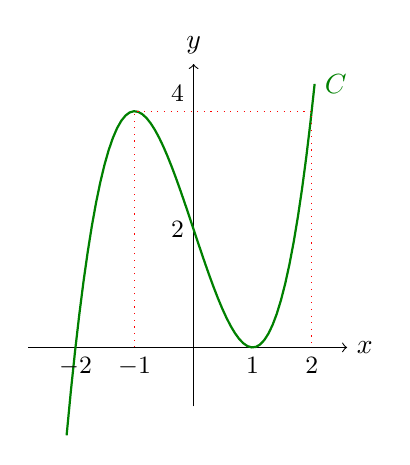
\begin{tikzpicture}[scale=0.75]
  \draw[->] (-2.8,0) -- (2.6,0) node[right] {$x$};
  \draw[->] (0,-1) -- (0,4.8) node[above] {$y$};
  \draw[thick,green!50!black,domain=-2.15:2.05,samples=60] plot (\x,{(\x)^3-3*\x+2}) node[right] {$C$};
  \draw[dotted,red] (-1,0) -- (-1,4) -- (2,4) -- (2,0);
  \foreach \x in {-2,-1,1,2} \node[below] at (\x,0) {\small $\x$};
  \node[above left] at (0,4) {\small $4$}; \node[left] at (0,2) {\small $2$};
\end{tikzpicture}
\end{center}
\begin{enumerate}[a]
  \item តាមក្រាប គ្រប់ចំណុច $(x, y)$ នៃក្រាបដែលមាន $y < 0$ ត្រូវស្ថិតនៅផ្នែកខាងក្រោមអ័ក្សអាប់ស៊ីស ហើយត្រូវគ្នានឹង $x < -2$ ។ ដូច្នេះ វិសមីការមានសំណុំចម្លើយ $S = (-\infty, -2)$ ។
  \item \textbf{របៀបទី $1$} ៖ តាមក្រាប ចំណុច $(x, y)$ នៃក្រាបដែលមាន $x \in [-2, 2]$ ត្រូវស្ថិតលើក្រាបដែលនៅខាងលើអ័ក្សអាប់ស៊ីស ជួបអ័ក្សអាប់ស៊ីសត្រង់ $x = -2$ និង $x = 1$ ហើយជួបបន្ទាត់ $y = 4$ ត្រង់ $x = -1$ និង $x = 2$ ។ ដូច្នេះ $0 \le y = x^3 - 3x + 2 \le 4$ ចំពោះ $x \in [-2, 2]$ ។

  \textbf{របៀបទី $2$} ៖ ដោយមិនប្រើក្រាប (ករណីគ្មានក្រាប) ៖ ប្រើតារាងអថេរភាព ។ ដេរីវេ $y' = 3x^2 - 3$ ។ បើ $y' = 0$, $3x^2 - 3 = 0 \Leftrightarrow x = \pm 1$ ។ តម្លៃបរមា ៖ $y(-1) = 4$, $y(1) = 0$ ។
  \begin{center}
  \begin{tikzpicture}
    \tkzTabInit[lgt=1.4,espcl=1.6]{$x$ /0.8, $y'$ /0.8, $y$ /1.6}{$-\infty$, $-2$, $-1$, $1$, $2$, $+\infty$}
    \tkzTabLine{, +, t, +, z, -, z, +, t, +, }
    \tkzTabVar{-/$-\infty$, R/, +/$4$, -/$0$, R/, +/$+\infty$}
    \tkzTabVal{1}{3}{0.5}{}{$0$}
    \tkzTabVal{4}{6}{0.5}{}{$4$}
  \end{tikzpicture}
  \end{center}
  តាមតារាងអថេរភាពនៃអនុគមន៍ខាងលើ គេបាន ៖ $0 \le y = x^3 - 3x + 2 \le 4$ ចំពោះ $x \in [-2, 2]$ ។
\end{enumerate}

\begin{formulaBox}[ជាទូទៅ]
\begin{itemize}
  \item វិសមីការ $ax^3 + bx^2 + cx + d > 0$ មានសំណុំឫសជាសំណុំតម្លៃអាប់ស៊ីស $x$ នៃចំណុចនៅលើក្រាបតាងអនុគមន៍ $y = ax^3 + bx^2 + cx + d$ ដែលស្ថិតនៅផ្នែកខាងលើអ័ក្សអាប់ស៊ីស ។
  \item វិសមីការ $ax^3 + bx^2 + cx + d < 0$ មានសំណុំឫសជាសំណុំតម្លៃអាប់ស៊ីស $x$ នៃចំណុចនៅលើក្រាបតាងអនុគមន៍ $y = ax^3 + bx^2 + cx + d$ ដែលស្ថិតនៅផ្នែកខាងក្រោមអ័ក្សអាប់ស៊ីស ។
\end{itemize}
\end{formulaBox}

\begin{pro}
អនុគមន៍ $y = -x^3 + 3x - 2$ មានក្រាប $C$ ។ \quad ក. រកសំណុំឫសនៃវិសមីការ $-x^3 + 3x - 2 \le 0$ តាមក្រាប ។ \quad ខ. បង្ហាញថា $-4 \le -x^3 + 3x - 2 \le 0$ ចំពោះ $-2 \le x \le 2$ ។
\ans
ក. $-x^3 + 3x - 2 = -(x - 1)^2(x + 2) \le 0$ ៖ $x \in [-2, +\infty)$ \quad ខ. លើ $[-2, 2]$ អនុគមន៍មានតម្លៃធំបំផុត $y(-2) = y(1) = 0$ និងតម្លៃតូចបំផុត $y(-1) = y(2) = -4$ ។
\end{pro}

\subsection{ការអនុវត្តដេរីវេចំពោះវិសមីការដែលអង្គទី 1 ជាកន្សោមប៊ីការេ}

\begin{example}[ឧទាហរណ៍]
គេឱ្យក្រាប $C$ នៃ $y = -x^4 - 2x^2 + 3$ ។ រកសំណុំឫសនៃវិសមីការ $-x^4 - 2x^2 + 3 \ge 0$ តាមក្រាបហ្វិក ។
\end{example}
តាមក្រាប ចំណុច $(x, y)$ នៃក្រាបដែលមាន $y \ge 0$ ត្រូវស្ថិតនៅផ្នែកខាងលើ ឬជួបនឹងអ័ក្សអាប់ស៊ីស ហើយត្រូវគ្នានឹង $-1 \le x \le 1$ ។ ដូច្នេះ វិសមីការមានសំណុំឫស $S = [-1, 1]$ ។

\begin{center}
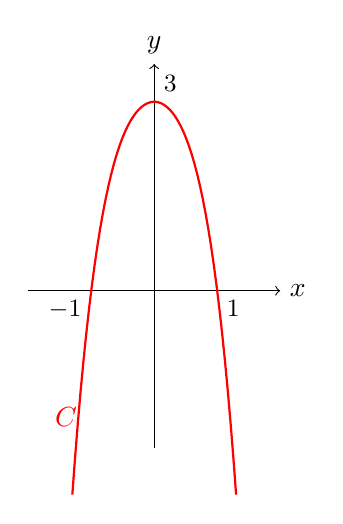
\begin{tikzpicture}[scale=0.8]
  \draw[->] (-2,0) -- (2,0) node[right] {$x$};
  \draw[->] (0,-2.5) -- (0,3.6) node[above] {$y$};
  \draw[thick,red,domain=-1.3:1.3,samples=60] plot (\x,{-(\x)^4-2*(\x)^2+3});
  \node[below left] at (-1,0) {\small $-1$}; \node[below right] at (1,0) {\small $1$};
  \node[above right] at (0,3) {\small $3$}; \node[red] at (-1.4,-2) {$C$};
\end{tikzpicture}
\end{center}

\begin{example}[លំហាត់គំរូ]
អនុគមន៍ $y = -\dfrac{1}{2}x^4 + 3x^2 - \dfrac{5}{2}$ មានក្រាប $C$ ។
\begin{enumerate}[a]
  \item ដោះស្រាយវិសមីការ $-\dfrac{1}{2}x^4 + 3x^2 - \dfrac{5}{2} < 0$ តាមក្រាប ។
  \item បង្ហាញថា $0 < -\dfrac{1}{2}x^4 + 3x^2 - \dfrac{5}{2} \le 2$ ចំពោះ $x \in (-\sqrt{5}, -1) \cup (1, \sqrt{5})$ តាមក្រាប ។
\end{enumerate}
\end{example}
\ans
\begin{center}
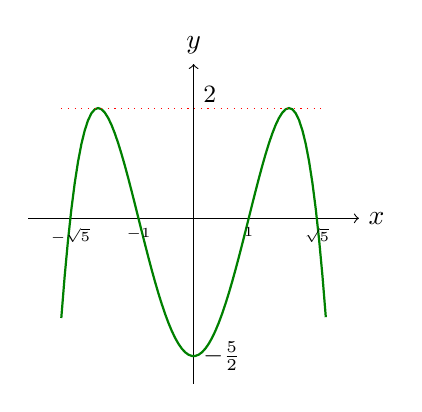
\begin{tikzpicture}[scale=0.7]
  \draw[->] (-3,0) -- (3,0) node[right] {$x$};
  \draw[->] (0,-3) -- (0,2.8) node[above] {$y$};
  \draw[thick,green!50!black,domain=-2.4:2.4,samples=80] plot (\x,{-0.5*(\x)^4+3*(\x)^2-2.5}) ;
  \draw[dotted,red] (-2.4,2) -- (2.4,2);
  \foreach \x/\l in {-2.236/-\sqrt{5},-1/-1,1/1,2.236/\sqrt{5}} \node[below] at (\x,0) {\tiny $\l$};
  \node[right] at (0,2.25) {\small $2$}; \node[right] at (0,-2.5) {\small $-\frac{5}{2}$};
\end{tikzpicture}
\end{center}
\begin{enumerate}[a]
  \item តាមក្រាប វិសមីការ $-\dfrac{1}{2}x^4 + 3x^2 - \dfrac{5}{2} < 0$ មានសំណុំឫស $S = (-\infty, -\sqrt{5}) \cup (-1, 1) \cup (\sqrt{5}, +\infty)$ ។
  \item តាមក្រាប ចំណុច $(x, y)$ នៃក្រាប $C$ ដែលមាន $0 < y \le 2$ ត្រូវស្ថិតនៅផ្នែកខាងលើអ័ក្សអាប់ស៊ីស ហើយប៉ះនឹងបន្ទាត់ $y = 2$ ដែលត្រូវគ្នានឹង $x \in (-\sqrt{5}, -1) \cup (1, \sqrt{5})$ ។ ដូច្នេះ $0 < -\dfrac{1}{2}x^4 + 3x^2 - \dfrac{5}{2} \le 2$ ចំពោះ $x \in (-\sqrt{5}, -1) \cup (1, \sqrt{5})$ ។
\end{enumerate}

\begin{formulaBox}[ជាទូទៅ]
\begin{itemize}
  \item វិសមីការ $ax^4 + bx^2 + c > 0$ មានសំណុំឫសជាសំណុំតម្លៃអាប់ស៊ីស $x$ នៃចំណុចនៅលើក្រាបតាងអនុគមន៍ $y = ax^4 + bx^2 + c$ ដែលស្ថិតនៅផ្នែកខាងលើអ័ក្សអាប់ស៊ីស ។
  \item វិសមីការ $ax^4 + bx^2 + c < 0$ មានសំណុំឫសជាសំណុំតម្លៃអាប់ស៊ីស $x$ នៃចំណុចនៅលើក្រាបតាងអនុគមន៍ $y = ax^4 + bx^2 + c$ ដែលស្ថិតនៅផ្នែកខាងក្រោមអ័ក្សអាប់ស៊ីស ។
\end{itemize}
\end{formulaBox}

\begin{pro}
អនុគមន៍ $y = x^4 - 2x^2 + 1$ មានក្រាប $C$ ។ \quad ក. ដោះស្រាយវិសមីការ $x^4 - 2x^2 + 1 > 0$ តាមក្រាប ។ \quad ខ. បង្ហាញថា $0 \le x^4 - 2x^2 + 1 \le 1$ ចំពោះ $x \in [-\sqrt{2}, \sqrt{2}]$ ។
\ans
ក. $x \in \mathbb{R} - \{\pm 1\}$ \quad ខ. លើ $[-\sqrt{2}, \sqrt{2}]$ អនុគមន៍មានតម្លៃតូចបំផុត $y(\pm 1) = 0$ និងតម្លៃធំបំផុត $y(0) = y(\pm\sqrt{2}) = 1$ ។
\end{pro}

\section*{មេរៀនសង្ខេប ជំពូកទី ៥}
\begin{note}[មេរៀនសង្ខេប]
\begin{enumerate}[1]
  \item បើ $x \to a$ ហើយ $f(x) \to b$ នោះកំណត់សរសេរដោយ $\displaystyle\lim_{x \to a} f(x) = b$ ។
  \item $\displaystyle\lim_{x \to a} c = c$ ចំពោះគ្រប់ចំនួនថេរ $c$ ។ \quad $\displaystyle\lim_{x \to a} x = a$ ។
  \item $\displaystyle\lim_{x \to a}[f(x) \pm g(x)] = \lim_{x \to a} f(x) \pm \lim_{x \to a} g(x)$ ។ \quad $\displaystyle\lim_{x \to a}[f(x)\times g(x)] = \lim_{x \to a} f(x)\times\lim_{x \to a} g(x)$ ។
  \item $\displaystyle\lim_{x \to a}\frac{f(x)}{g(x)} = \frac{\lim_{x \to a} f(x)}{\lim_{x \to a} g(x)}$ បើ $\displaystyle\lim_{x \to a} g(x) \ne 0$ ។
  \item បើ $\displaystyle\lim_{x \to x_0^-} f(x) = L$ នោះ $L$ ជាលីមីតខាងឆ្វេងនៃ $y = f(x)$ ។ បើ $\displaystyle\lim_{x \to x_0^+} f(x) = R$ នោះ $R$ ជាលីមីតខាងស្ដាំនៃ $y = f(x)$ ។ $f$ មានលីមីតត្រង់ $x_0$ លុះត្រាតែ $\displaystyle\lim_{x \to x_0^-} f(x) = \lim_{x \to x_0^+} f(x)$ ។
  \item លីមីតនៃអនុគមន៍ពហុធានៅត្រង់អនន្ត គឺជាលីមីតនៃតួដែលមានដឺក្រេធំជាងគេ ។ លីមីតនៃអនុគមន៍សនិទាននៅត្រង់អនន្ត គឺជាផលធៀបរវាងលីមីតនៃតួដែលមានដឺក្រេធំជាងគេនៅភាគយក និងលីមីតនៃតួដែលមានដឺក្រេធំជាងគេនៅភាគបែង ។
  \item ផលធៀប $\dfrac{\Delta y}{\Delta x} = \dfrac{f(b) - f(a)}{b - a}$ ជាអត្រាបម្រែបម្រួលមធ្យមនៃ $y = f(x)$ កាលណា $x$ បម្រែបម្រួលពី $a$ ទៅ $b$ ។
  \item $f'(a) = \displaystyle\lim_{h \to 0}\frac{f(a + h) - f(a)}{h}$ ជាដេរីវេនៃអនុគមន៍ $y = f(x)$ នៅត្រង់ $x = a$ ។
  \item $(c)' = 0$ ចំពោះគ្រប់ចំនួនថេរ $c$ ។ $(x^n)' = nx^{n-1}$ ចំពោះ $n \in \mathbb{N}$ និង $r \in \mathbb{Q}$, $(x^r)' = rx^{r-1}$ ។ $[kf(x)]' = kf'(x)$ ដែល $k$ ជាមេគុណថេរ ។
  \item $[f(x) \pm g(x)]' = f'(x) \pm g'(x)$ ។ $[f(x)\times g(x)]' = f'(x)\times g(x) + f(x)\times g'(x)$ ។ $\left[\dfrac{f(x)}{g(x)}\right]' = \dfrac{f'(x)\times g(x) - f(x)\times g'(x)}{[g(x)]^2}$ បើ $g(x) \ne 0$ ។
  \item $f''(x)$ ជាដេរីវេទី $1$ នៃ $f'(x)$ ហើយ $f''(x)$ ជាដេរីវេទី $2$ នៃអនុគមន៍ $y = f(x)$ ។
  \item មេគុណប្រាប់ទិសនៃបន្ទាត់ប៉ះនឹងក្រាបតាង $f$ ត្រង់ $(x_0, y_0)$ ៖ $m = \displaystyle\lim_{x \to x_0}\frac{f(x) - f(x_0)}{x - x_0} = \frac{dy}{dx}(x_0) = f'(x_0)$ ។ សមីការបន្ទាត់ប៉ះ ៖ $y - y_0 = f'(x_0)(x - x_0)$ ឬ $y = f'(x_0)(x - x_0) + y_0$ ។
  \item ទិសដៅអថេរភាពនៃអនុគមន៍ ៖ $f$ កើនលើ $(a, b)$ លុះត្រាតែ $f'(x) > 0$, ចុះលើ $(a, b)$ លុះត្រាតែ $f'(x) < 0$, ថេរលើ $(a, b)$ លុះត្រាតែ $f'(x) = 0$ គ្រប់ $x \in (a, b)$ ។
  \item អតិបរមាធៀបនិងអប្បបរមាធៀបនៃអនុគមន៍តាមដេរីវេទី $1$ ៖ $f$ មានអតិបរមាធៀបត្រង់ $x_0$ កាលណា $f'$ ដូរសញ្ញាពី $+$ ទៅ $-$ ត្រង់ $x_0$ ។ $f$ មានអប្បបរមាធៀបត្រង់ $x_0$ កាលណា $f'$ ដូរសញ្ញាពី $-$ ទៅ $+$ ត្រង់ $x_0$ ។
  \item អតិបរមាធៀបនិងអប្បបរមាធៀបតាមដេរីវេទី $2$ ៖ $f$ មានអតិបរមាធៀបត្រង់ $x_0$ កាលណា $f'(x_0) = 0$ និង $f''(x_0) < 0$ ។ $f$ មានអប្បបរមាធៀបត្រង់ $x_0$ កាលណា $f'(x_0) = 0$ និង $f''(x_0) > 0$ ។
  \item ចំណុច $I(x_0, y_0)$ ជាចំណុចរបត់នៃខ្សែកោងតាង $f$ កាលណាខ្សែកោងប៉ោងឬផតលើ $[a, x_0]$ ហើយផតឬប៉ោងលើ $[x_0, b]$ ។ របៀបរក ៖ រក $f''(x)$, ដោះស្រាយ $f''(x) = 0$ និងសិក្សាសញ្ញានៃ $f''(x)$ ។
  \item ល្បឿននៃចលនា ៖ ចំណុច $M(x = f(t))$ មានល្បឿននៅខណៈពេល $t$ គឺ $V = \dfrac{dx}{dt} = f'(t)$ ។
  \item ចំណុចរបត់ជាផ្ចិតឆ្លុះនៃក្រាបតាងអនុគមន៍ដឺក្រេទី $3$ ។ អ័ក្សអរដោនេជាអ័ក្សឆ្លុះនៃក្រាបតាងអនុគមន៍ $y = ax^4 + bx^2 + c$ ។
  \item អាស៊ីមតូត ៖ បន្ទាត់ $x = x_0$ ជាអាស៊ីមតូតឈរនៃក្រាបតាង $y = f(x)$ កាលណា $\displaystyle\lim_{x \to x_0} f(x) = \pm\infty$ ។ បន្ទាត់ $y = b$ ជាអាស៊ីមតូតដេកកាលណា $\displaystyle\lim_{x \to \pm\infty} f(x) = b$, $b \in \mathbb{R}$ ។
  \item ចំណុច $S\left(-\dfrac{d}{c}, \dfrac{a}{c}\right)$ ជាផ្ចិតឆ្លុះនៃក្រាបតាងអនុគមន៍ $y = \dfrac{ax + b}{cx + d}$ ហើយជាចំណុចប្រសព្វរវាងអាស៊ីមតូតឈរនិងដេក ។
  \item សមីការ $ax^3 + bx^2 + cx + d = \lambda$ (ឬ $ax^4 + bx^2 + c = \lambda$) មានឫសជាអាប់ស៊ីសនៃចំណុចប្រសព្វរវាងក្រាបនៃអនុគមន៍ និងបន្ទាត់ $y = \lambda$ ។
  \item វិសមីការ $f(x) > 0$ (ឬ $f(x) < 0$) មានសំណុំឫសជាសំណុំតម្លៃអាប់ស៊ីស $x$ នៃចំណុចនៅលើក្រាបតាង $f$ ដែលស្ថិតនៅផ្នែកខាងលើ (ឬខាងក្រោម) អ័ក្សអាប់ស៊ីស ។ ក្នុងការដោះស្រាយវិសមីការដឺក្រេទី $3$ ឬទី $4$ គេអាចប្រើក្រាប ឬតារាងអថេរភាពនៃអនុគមន៍ ។
\end{enumerate}
\end{note}

\section*{លំហាត់ជំពូកទី ៥}
\begin{enumerate}[1]
  \item $f$ ជាអនុគមន៍កំណត់ដោយ $f(x) = \dfrac{3x^2 - 4x - 4}{x^2 - x - 2}$ បើ $x > 2$, $f(x) = \dfrac{\sqrt{x^2 + 5} - 3}{\sqrt{x + 2} - 2}$ បើ $x < 2$ និង $f(2) = \dfrac{8}{3}$ ។ គណនា $\displaystyle\lim_{x \to +\infty} f(x)$, $\displaystyle\lim_{x \to -2^+} f(x)$, $\displaystyle\lim_{x \to 2^+} f(x)$ និង $\displaystyle\lim_{x \to 2^-} f(x)$ ។
  \item គេឱ្យអនុគមន៍ $f(x) = \begin{cases} 5 - ax^2 & \text{បើ } x > 2\\ x + 1 & \text{បើ } x \le 2 \end{cases}$ ។ កំណត់តម្លៃ $a$ ដើម្បីឱ្យ $f$ មានលីមីតត្រង់ $x = 2$ ។
  \item គេឱ្យអនុគមន៍ $f(x) = \begin{cases} \dfrac{\sqrt{x} - 1}{x - 1} & \text{បើ } x > 1\\ \dfrac{m^2 + m - 7}{2} + 2x - 2 & \text{បើ } x \le 1 \end{cases}$ ។ តើតម្លៃ $m$ ស្មើប៉ុន្មានដែលធ្វើឱ្យ $f$ ជាអនុគមន៍មានលីមីតត្រង់ $x = 1$ ។
  \item គណនាលីមីតខាងក្រោម ៖
  \begin{tasks}(3)
    \task $\displaystyle\lim_{x \to 3}\frac{x^2 - 5x + 6}{9 - x^2}$
    \task $\displaystyle\lim_{x \to -5}\frac{x^2 + 6x + 5}{x^2 + 4x - 5}$
    \task $\displaystyle\lim_{x \to 2}\frac{x^3 - 8}{x^2 - 2x}$
    \task $\displaystyle\lim_{x \to 2}\frac{x^3 - 2x^2 - 4x + 8}{x^3 - 4x^2 + 4x}$
    \task $\displaystyle\lim_{x \to 5}\frac{\sqrt{x - 1} - 2}{x - 5}$
    \task $\displaystyle\lim_{x \to 4}\frac{\sqrt{2x + 1} - 3}{\sqrt{x} - 2}$
  \end{tasks}
  \item គណនាលីមីតខាងក្រោម ៖
  \begin{tasks}(2)
    \task $\displaystyle\lim_{x \to 2}\frac{\sqrt{x + 2} - 2}{x - 2}$
    \task $\displaystyle\lim_{x \to 3}\frac{\sqrt{2x + 3} - \sqrt{x + 6}}{\sqrt{x - 1} - \sqrt{8 - 2x}}$
    \task $\displaystyle\lim_{x \to 3}\frac{x^2 - x - 6}{\sqrt{x + 6} - 3}$
    \task $\displaystyle\lim_{x \to 4}\frac{\sqrt{x + 5} - \sqrt{x - 1}}{\sqrt{x + 12} - \sqrt{x} - 2}$
    \task $\displaystyle\lim_{x \to 1}\frac{1}{x - 1}\left(x + 1 + \frac{2}{x - 2}\right)$
    \task $\displaystyle\lim_{x \to 0}\frac{x^2 + 3x}{|x|}$
  \end{tasks}
  \item គណនាលីមីតខាងក្រោម ៖
  \begin{tasks}(2)
    \task $\displaystyle\lim_{x \to +\infty}\frac{1 + 2\sqrt{x} - x}{x + 2}$
    \task $\displaystyle\lim_{x \to -\infty}\frac{\sqrt{x^2 + 5x} - 3}{2x + 1}$
    \task $\displaystyle\lim_{x \to \infty}\frac{(x - 1)^2(7x^2 + 2)}{(2x + 3)^4}$
    \task $\displaystyle\lim_{x \to +\infty}(x - \sqrt{x^2 + 3})$
    \task $\displaystyle\lim_{x \to -\infty}(\sqrt{x^2 + 2x} + x - 1)$
    \task $\displaystyle\lim_{x \to +\infty}(x + 1 - \sqrt{x^2 + 3x})$
  \end{tasks}
  \item គណនាដេរីវេនៃអនុគមន៍ខាងក្រោម ៖
  \begin{tasks}(2)
    \task $y = (x^2 + 1)(x^3 - 2x + 4)$
    \task $y = \dfrac{1}{x^4} + 2\sqrt{x} + \dfrac{7}{\sqrt[3]{x}}$
    \task $y = \dfrac{x^2 + 2x - 2}{x^2 + 1}$
    \task $y = \dfrac{1}{(x^2 + x + 1)^2}$
    \task $y = x\sqrt{x} + \sqrt[5]{x^3}$
    \task $y = (x^2 + 3x - 2)^{10}$
  \end{tasks}
  \item គណនាដេរីវេនៃអនុគមន៍ខាងក្រោម ៖
  \begin{tasks}(2)
    \task $y = \sqrt{9 - x^2}$
    \task $y = (x^2 - x)^2(x + 1)$
    \task $y = \sqrt{\dfrac{x - 1}{x + 1}}$
    \task $y = x\sqrt[3]{1 + x^2}$
  \end{tasks}
  \item កំណត់តម្លៃ $a$ ដើម្បីឱ្យលីមីត $\displaystyle\lim_{x \to 2}\frac{\sqrt{x + a} - 3}{x^2 - 5x + 6}$ ជាចំនួនកំណត់ ។
  \item កំណត់តម្លៃ $a$ និង $b$ ដើម្បីឱ្យលីមីត $\displaystyle\lim_{x \to 8}\frac{ax^2 + bx + 8}{\sqrt[3]{x} - 2} = 84$ ។
  \item រកតម្លៃអតិបរមាធៀបនិងអប្បបរមាធៀបនៃអនុគមន៍ខាងក្រោម ៖ \quad ក. $y = x^3 + 3x^2 - 9x + 1$ \quad ខ. $y = x^4 - 4x^2 + 5$ ។
  \item រកតម្លៃ $m$ ដើម្បីឱ្យអនុគមន៍ $y = 2x^3 + 3(m - 1)x^2 + 6(m - 2)x - 1$ មានអតិបរមាធៀបមួយនិងអប្បបរមាធៀបមួយ ។
  \item រកចំណុចរបត់នៃអនុគមន៍ខាងក្រោម ៖
  \begin{tasks}(2)
    \task $y = x^3 - 8$
    \task $y = -\dfrac{x^3}{3} + 3x^2 - 9x + 5$
    \task $y = x^3 + 6x^2 + 9x + 7$
    \task $y = -\dfrac{x^4}{12} + 2x^2 - 3$
  \end{tasks}
  \item គេឱ្យអនុគមន៍ $y = (m^2 - 2)x^3 + (m + 4)x^2$ ។ \quad ក. កំណត់តម្លៃ $m$ ដើម្បីឱ្យអនុគមន៍នេះមាន $I(1, 2)$ ជាចំណុចរបត់ ។ \quad ខ. ចំពោះតម្លៃ $m$ ដែលបានរកឃើញ ចូរសិក្សាអថេរភាពនិងសង់ក្រាប $C$ តាងអនុគមន៍នេះ ។
  \item សិក្សាអថេរភាពនិងសង់ក្រាប $C$ តាងអនុគមន៍ $y = x^3 - 3x^2 - 6x + 8$ ។
  \item សិក្សាអថេរភាពនិងសង់ក្រាប $C$ តាងអនុគមន៍ $y = \dfrac{2x - 1}{x + 2}$ ។
  \item សិក្សាអថេរភាពនិងសង់ក្រាបតាងអនុគមន៍ខាងក្រោម ៖
  \begin{tasks}(2)
    \task $y = x^3 - 3x$
    \task $y = -x^3 + 6x^2 - 9x + 4$
    \task $y = x^4 - 5x^2 + 4$
    \task $y = -x^4 + 3x^2 - 5$
    \task $y = \dfrac{2x - 2}{x - 2}$
    \task $y = \dfrac{3 - 2x}{x + 1}$
  \end{tasks}
  \item គេឱ្យអនុគមន៍ $f(x) = x^2$ និង $h$ ជាចំនួនពិតខុសពីសូន្យ ។ រកតម្លៃ $\alpha$ ដើម្បីឱ្យ $f(x_0 + h) = f(x_0) + h\cdot f'(x_0 + \alpha h)$ ។
  \item បន្ទាត់ $T$ មួយប៉ះនឹងក្រាបនៃអនុគមន៍ $y = x^3$ ត្រង់ចំណុច $M$ មួយ ហើយជួបអ័ក្សអាប់ស៊ីសនិងអ័ក្សអរដោនេរៀងគ្នាត្រង់ចំណុច $A$ និង $B$ ។ រកផលធៀប $AM : BM$ ។
  \item គេឱ្យអនុគមន៍ $y = 6x^5 - 15x^4 + 10x^3 - 2$ ។ \quad ក. គណនា $y'$ និងសិក្សាសញ្ញានៃ $y'$ ។ \quad ខ. សង់តារាងអថេរភាព និងក្រាបនៃអនុគមន៍ $y$ ។
  \item ប៉ារ៉ាបូលតាង $y = 9 - x^2$ កាត់អ័ក្សអាប់ស៊ីសត្រង់ចំណុច $E$ និង $F$ ។ ចតុកោណព្នាយ $EFGH$ ចារឹកក្នុងប៉ារ៉ាបូល ហើយមានអង្កត់ $EF$ ជាបាតធំ និង $GH$ ជាបាតតូច ។ \quad ក. រកកូអរដោនេនៃចំណុច $G$ និង $H$ ដើម្បីឱ្យចតុកោណព្នាយមានផ្ទៃក្រឡាធំបំផុត ។ \quad ខ. គណនាផ្ទៃក្រឡាធំបំផុតនោះ ។
  \item ក. ក្រាប $C_1$ នៃអនុគមន៍ $y = x^3 + ax$ និង $C_2$ នៃ $y = x^2 + bx + c$ កាត់គ្នាត្រង់ $A(1, 2)$ ហើយមានបន្ទាត់ប៉ះរួមត្រង់ចំណុចនោះ ។ រកតម្លៃ $a, b$ និង $c$ ។ \quad ខ. ចំពោះតម្លៃនៃចំនួនពិត $a, b$ និង $c$ ដែលរកឃើញ សង់ក្រាប $C_1$, $C_2$ និងបន្ទាត់ប៉ះរួមត្រង់ $A$ ។
  \item ក. រកតម្លៃ $k$ ដើម្បីឱ្យអនុគមន៍ $f(x) = x^3 - 4x^2 + 2kx$ គ្មានបរមា ។ \quad ខ. រកតម្លៃ $a$ ដើម្បីឱ្យអនុគមន៍ $y = x^4 + 2ax^2 + a$ មានអតិបរមា និងអប្បបរមា ។
  \item រកតម្លៃអតិបរមា និងអប្បបរមានៃអនុគមន៍ $y = 2x^3 - 3ax^2 + 1$ លើចន្លោះ $0 \le x \le 3$ ដែល $a > 0$ ។
  \item គេឱ្យចតុមុខនិយ័ត $ABCD$ មួយដែលមានទ្រនុង $12$ cm ។ ចំណុច $M, N, P$ ស្ថិតនៅលើទ្រនុង $AB, AC, AD$ រៀងគ្នា ហើយមានចម្ងាយ $x$ ដូចគ្នាពីកំពូល $A$ ។ ចំណុច $M', N', P'$ ជាចំណោលកែងនៃ $M, N, P$ រៀងគ្នាទៅលើបាត $BCD$ ។ រកតម្លៃ $x$ បើគេដឹងថាព្រីសត្រីមុខនិយ័ត $MNP\cdot M'N'P'$ មានមាឌធំបំផុត ។
  \item គេឱ្យសមីការ $2x^3 - 3x^2 - 12x - k = 0$ \ $(E)$ ។ \quad ក. រកតម្លៃ $k$ ដើម្បីឱ្យ $(E)$ មានឫសបីផ្សេងគ្នា ។ \quad ខ. ដោះស្រាយវិសមីការ $2x^3 - 3x^2 - 12x - k \le 0$ តាមក្រាប ។
  \item អនុគមន៍ $f(x) = x^2(6 - 3x^2)$ មានក្រាប $C$ ។ \quad ក. រកតម្លៃ $P$ ដើម្បីឱ្យសមីការ $f(x) = P$ មានឫសបួនផ្សេងគ្នាតាមក្រាប ។ \quad ខ. បង្ហាញថា $0 \le 6x^2 - 3x^4 < 3$ ចំពោះ $x \in (-1, 1)$ ។
  \item គណនាលីមីតខាងក្រោម ៖
  \begin{tasks}(3)
    \task $\displaystyle\lim_{x \to 1}[(x^2 + 4x + 2)(3 - x^2)]$
    \task $\displaystyle\lim_{x \to -2}\frac{3x^2 - x - 4}{(2x + 5)^2}$
    \task $\displaystyle\lim_{x \to 1}\frac{2x^2 - 5x + 3}{x^2 + x - 2}$
    \task $\displaystyle\lim_{x \to 0}\frac{x^2 + x}{|x|}$
    \task $\displaystyle\lim_{x \to 0}\frac{2x^2 + |x|}{|x|}$
    \task $\displaystyle\lim_{x \to 3}\frac{x}{x^2 + 1}$
    \task $\displaystyle\lim_{x \to 3}\frac{x^3 - 27}{x - 3}$
    \task $\displaystyle\lim_{x \to -1}\frac{x^2 + 3x + 2}{x^2 - 2x - 3}$
    \task $\displaystyle\lim_{x \to 1}\frac{x^{100} - 7x + 6}{x^{50} + 3x - 4}$
    \task $\displaystyle\lim_{x \to 1}\frac{x^3 - 4x + 3}{x^3 - x^2 + 2x - 2}$
    \task $\displaystyle\lim_{x \to 1}\frac{\sqrt{2x - 1} - 1}{x - 1}$
    \task $\displaystyle\lim_{x \to 1}\frac{3x - 3}{1 + \sqrt[3]{x - 2}}$
    \task $\displaystyle\lim_{x \to 0}\frac{\sqrt[m]{ax + 1}\,\sqrt[n]{bx + 1} - 1}{x}$
    \task $\displaystyle\lim_{x \to \pm\infty}\frac{x^2 - 1}{x^2 + 3}$
    \task $\displaystyle\lim_{x \to +\infty}\frac{-x^2 + x + 1}{2x + 1}$
    \task $\displaystyle\lim_{x \to \pm\infty}\frac{\sqrt{4x^2 + 3} - 2x}{\sqrt{x^2 + 4} + 2x}$
    \task $\displaystyle\lim_{x \to +\infty}(\sqrt{x^2 + x + 1} - x)$
    \task $\displaystyle\lim_{x \to -\infty}(\sqrt{4x^2 + 4} + x)$
    \task $\displaystyle\lim_{x \to +\infty}(\sqrt{x^2 + 3} - \sqrt{x^2 - 2x})$
  \end{tasks}
  \item ក. គេឱ្យ $f(x) = x^2 - 2x$ ។ ចូរគណនា $\displaystyle\lim_{x \to 1}\frac{f(x) - f(1)}{x - 1}$ ។ \quad ខ. $f$ ជាអនុគមន៍កំណត់ដោយ $f(x) = ax^2 + bx + c$ ។ ចូររក $\displaystyle\lim_{x \to a}\frac{f(x) - f(a)}{x - a}$ ។
  \item គណនាដេរីវេនៃអនុគមន៍ខាងក្រោម ៖
  \begin{tasks}(2)
    \task $f(x) = \dfrac{1}{3}x^3 - \dfrac{1}{2}x^2 + 5x$
    \task $f(x) = (2x - 3)(3x + 2)$
    \task $f(x) = (2x^2 - 5)^2$
    \task $y = (2x^3 + 1)^5 + (x^2 - 3)^3$
    \task $y = \dfrac{2x - 3}{5x + 1}$
    \task $y = (2x^2 - 3)(3x^2 + 2)$
    \task $y = \dfrac{2x^2 - 3x + 4}{x - 2}$
    \task $y = \dfrac{-3x^2 + 5x + 4}{3x - 2}$
  \end{tasks}
  \item ក. គណនា $f'(x)$ និង $f'(1)$ នៃអនុគមន៍ $f(x) = \dfrac{x^4}{2} + 2x$ ។ \quad ខ. គណនាដេរីវេ $y'$, $y'(0)$ និង $y'(1)$ នៃអនុគមន៍ $y = \sqrt[3]{x^2 - 4x + 3}$ ។ \quad គ. គណនាដេរីវេ $\dfrac{dy}{dx}$ និង $\dfrac{dy}{dx}\left(\dfrac{1}{2}\right)$ នៃអនុគមន៍ $y = x^5 - x^4 + 4x^2 - 3x + 2$ ។ \quad ឃ. គណនាដេរីវេ $y'(1)$ នៃអនុគមន៍ $y = \dfrac{x^2 - 3x + 5}{x - 3}$ ។ \quad ង. គណនាដេរីវេ $y'(0)$ នៃអនុគមន៍ $y = \dfrac{(5 - 2x)(2x + 1)}{3x - 2}$ ។
  \item ក. គេឱ្យអនុគមន៍ $y = \dfrac{x + 3}{x - 1}$ ។ គណនា $y'$ និង $y'(-1)$ ។ \quad ខ. គេឱ្យអនុគមន៍ $y = \dfrac{x + 1}{x^2}$ ។ គណនា $y'$ និង $y'(1)$ ។ \quad គ. គេឱ្យអនុគមន៍ $y = \dfrac{(x + 1)(2 - x)}{2x - 1}$ ។ គណនា $y'$ និង $y'(0)$ ។
  \item គេឱ្យអនុគមន៍ $f(x) = 2x^3 - 12x + 3$ ។ \quad ក. រកតម្លៃ $x$ ដើម្បីឱ្យ $f'(x) = 0$ \quad ខ. រកតម្លៃ $x$ ដើម្បីឱ្យ $f''(x) = 12$ ។
  \item គេឱ្យអនុគមន៍ $f(x) = x^3 - 3x^2 + 4x - 6$ ។ \quad ក. រកតម្លៃ $x$ ដើម្បីឱ្យ $f'(x) = 1$ \quad ខ. រកតម្លៃ $x$ ដើម្បីឱ្យ $f''(x) = 0$ ។
  \item អនុគមន៍ $f$ កំណត់ដោយ $f(x) = -4x^3 + x^2 + 14x - 1$ ។ \quad ក. រកតម្លៃ $x$ ដើម្បីឱ្យ $f'(x) = 0$ ហើយសិក្សាសញ្ញានៃ $f'(x)$ \quad ខ. រកតម្លៃ $x$ ដើម្បីឱ្យ $f''(x) = 0$ ហើយសិក្សាសញ្ញានៃ $f''(x)$ ។
  \item គេឱ្យក្រាប $C : y = f(x) = x^2 - x + 1$ ។ រកសមីការបន្ទាត់ប៉ះគូសពីចំណុច $A(1, 3)$ ប៉ះទៅនឹងក្រាប $C$ ។
  \item អនុគមន៍ $f(x) = x^3 - 6x^2 + 5$ មានក្រាប $C$ ។ \quad ក. រកសមីការបន្ទាត់ $L$ ដែលប៉ះក្រាប $C$ ត្រង់ចំណុចអាប់ស៊ីស $-2$ ។ \quad ខ. រកសមីការបន្ទាត់ដែលមានមេគុណប្រាប់ទិសស្មើ $-4$ ហើយប៉ះនឹងក្រាប $C$ ។
  \item ក. រកតម្លៃ $m$ ដើម្បីឱ្យអនុគមន៍ $y = x^3 + mx^2 - mx + 2$ មានអតិបរមានិងអប្បបរមាធៀប ។ \quad ខ. រកតម្លៃ $m$ ដើម្បីឱ្យអនុគមន៍ $y = x^3 + 2mx^2 + mx - 3$ មានអតិបរមានិងអប្បបរមាធៀប ។
  \item រកតម្លៃអតិបរមាធៀបនិងអប្បបរមាធៀបនៃអនុគមន៍ខាងក្រោម ៖ \quad ក. $f(x) = x^3 - 3x^2 - 2$ \quad ខ. $f(x) = -x^3 + 3x^2 + 2$ \quad គ. $f(x) = x^4 - 4x^2 + 2$ ។
  \item អនុគមន៍ $f(x) = x^3 + 3ax^2 + 3bx + 2$ មានអតិបរមាធៀបត្រង់ $x = 1$ និងអប្បបរមាធៀបត្រង់ $x = 2$ ។ \quad ក. រកតម្លៃនៃចំនួនពិត $a$ និង $b$ \quad ខ. រកផលដករវាងតម្លៃអតិបរមានិងអប្បបរមាធៀបនៃ $f$ ។
  \item អនុគមន៍ $f(x) = x^3 + ax^2 + bx + 4$ មានអតិបរមាធៀបត្រង់ $x = 0$ និងអប្បបរមាធៀបត្រង់ $x = 1$ ។ \quad ក. រកតម្លៃនៃចំនួនពិត $a$ និង $b$ \quad ខ. រកផលដករវាងតម្លៃអតិបរមានិងអប្បបរមាធៀបនៃ $f$ ។
  \item អនុគមន៍ $y = 3x^2 - 4x + 1$ កំណត់នៅលើ $\mathbb{R}$ និងមានក្រាប $(C)$ ។ \quad ក. រកសមីការបន្ទាត់ប៉ះនឹង $(C)$ ហើយកែងនឹងបន្ទាត់ $y = -\dfrac{x}{5} + 2$ ។ \quad ខ. រកសមីការបន្ទាត់ប៉ះនឹង $(C)$ ហើយស្របនឹងបន្ទាត់ $y = x + 5$ ។
  \item អនុគមន៍ $f(x) = 2x^3 - 16x + 11$ មានក្រាប $(C)$ ។ \quad ក. រកសមីការបន្ទាត់ $(L)$ ដែលប៉ះនឹងក្រាប $(C)$ ត្រង់ចំណុច $A(2, -5)$ ។ \quad ខ. រកសមីការបន្ទាត់ប៉ះដែលមានមេគុណប្រាប់ទិសស្មើ $-10$ ហើយប៉ះនឹងក្រាប $(C)$ ។
  \item គេឱ្យអនុគមន៍ $f(x) = 4x^3 + 9x^2 - 30x + 1$ មានក្រាប $(C)$ ។ \quad ក. គណនាលីមីតពេល $x$ ខិតជិត $1$ \quad ខ. គណនាដេរីវេទី $1$ នៃ $f(x)$ \quad គ. រកកូអរដោនេនៃគ្រប់ចំណុចប៉ះនៃក្រាប $(C)$ ដែលមានបន្ទាត់ប៉ះជាបន្ទាត់ដេក \quad ឃ. រកសមីការនៃបន្ទាត់ប៉ះទាំងនោះ ។
\end{enumerate}

\section*{លំហាត់អនុវត្តន៍}
\begin{enumerate}[1]
  \item អនុគមន៍ $y = x^3 - 3x^2$ មានក្រាប $C$ ។ \quad ក. សង់ក្រាប $C$ នៃអនុគមន៍ ។ \quad ខ. សិក្សាទៅតាមតម្លៃប៉ារ៉ាម៉ែត្រ $m$ នូវអត្ថិភាព និងចំនួនឫសនៃសមីការ $x^3 - 3x^2 = m$ តាមក្រាប ។
  \ans
  ក. អតិបរមាធៀប $y(0) = 0$, អប្បបរមាធៀប $y(2) = -4$ ។ ខ. បើ $m > 0$ ឬ $m < -4$ ៖ ឫស $1$ ។ បើ $m = 0$ ៖ ឫសឌុប $x = 0$ និងឫស $x = 3$ ។ បើ $-4 < m < 0$ ៖ ឫស $3$ ផ្សេងគ្នា ។ បើ $m = -4$ ៖ ឫសឌុប $x = 2$ និងឫស $x = -1$ ។
  \item អនុគមន៍ $f$ កំណត់ដោយ $f(x) = x^3 - 6x + 5$ ។ \quad ក. សង់ក្រាបនៃ $f$ ។ \quad ខ. សិក្សាលើក្រាបទៅតាមតម្លៃ $a$ នូវអត្ថិភាព និងសញ្ញាឫសនៃសមីការ $x^3 - 6x + 5 - a = 0$ ។
  \ans
  ក. អតិបរមាធៀប $f(-\sqrt{2}) = 5 + 4\sqrt{2}$, អប្បបរមាធៀប $f(\sqrt{2}) = 5 - 4\sqrt{2}$, $f(0) = 5$ ។ ខ. $a > 5 + 4\sqrt{2}$ ៖ ឫសវិជ្ជមានមួយ ។ $a = 5 + 4\sqrt{2}$ ៖ ឫសឌុបអវិជ្ជមាន និងឫសវិជ្ជមានមួយ ។ $5 < a < 5 + 4\sqrt{2}$ ៖ ឫសអវិជ្ជមានពីរ និងឫសវិជ្ជមានមួយ ។ $a = 5$ ៖ ឫស $0$, $\pm\sqrt{6}$ ។ $5 - 4\sqrt{2} < a < 5$ ៖ ឫសវិជ្ជមានពីរ និងឫសអវិជ្ជមានមួយ ។ $a = 5 - 4\sqrt{2}$ ៖ ឫសឌុបវិជ្ជមាន និងឫសអវិជ្ជមានមួយ ។ $a < 5 - 4\sqrt{2}$ ៖ ឫសអវិជ្ជមានមួយ ។
  \item គេឱ្យសមីការ $2x^3 - 3x^2 - 12x - k = 0$ ដែលមានអញ្ញាត $x$ និងប៉ារ៉ាម៉ែត្រ $k$ ។ \quad ក. រកតម្លៃ $k$ ដើម្បីឱ្យសមីការមានឫសបីផ្សេងគ្នា ។ \quad ខ. រកតម្លៃ $k$ ដើម្បីឱ្យសមីការមានឫសវិជ្ជមានពីរផ្សេងគ្នា និងឫសអវិជ្ជមានមួយទៀត ។
  \ans
  តាង $g(x) = 2x^3 - 3x^2 - 12x$ មានអតិបរមាធៀប $g(-1) = 7$ និងអប្បបរមាធៀប $g(2) = -20$ ។ ក. $-20 < k < 7$ \quad ខ. $-20 < k < 0$ ។
  \item អនុគមន៍ $f$ កំណត់ដោយ $f(x) = x^3 - 3x + 1$ មានក្រាប $C$ ។ \quad ក. សង់ក្រាប $C$ នៃ $f$ ។ \quad ខ. សិក្សាលើក្រាបទៅតាមតម្លៃ $p$ នូវអត្ថិភាព និងទីតាំងឫសនៃសមីការ $f(x) = p$ ធៀបនឹងចំនួន $-1$ និង $1$ ។
  \ans
  ក. អតិបរមាធៀប $f(-1) = 3$, អប្បបរមាធៀប $f(1) = -1$ ។ ខ. $p > 3$ ៖ $-1 < 1 < x_1$ ។ $p = 3$ ៖ $x_1 = x_2 = -1 < 1 < x_3$ ។ $-1 < p < 3$ ៖ $x_1 < -1 < x_2 < 1 < x_3$ ។ $p = -1$ ៖ $x_1 < -1 < 1 = x_2 = x_3$ ។ $p < -1$ ៖ $x_1 < -1 < 1$ ។
  \item ក. សង់ក្រាបនៃអនុគមន៍ $y = \dfrac{3}{2}x^4 + \dfrac{1}{2}x^2 - 4$ ។ \quad ខ. សិក្សាលើក្រាបទៅតាមតម្លៃ $m$ នូវអត្ថិភាព និងទីតាំងឫសនៃសមីការ $\dfrac{3}{2}x^4 + \dfrac{1}{2}x^2 - 4 - m = 0$ ធៀបនឹង $-1$ និង $2$ ។
  \ans
  ក. អប្បបរមា $y(0) = -4$ ។ $y(\pm 1) = -2$, $y(\pm 2) = 22$ ។ ខ. $m < -4$ ៖ គ្មានឫស ។ $m = -4$ ៖ ឫសឌុប $x = 0$ ។ $-4 < m < -2$ ៖ $-1 < x_1 < x_2 < 2$ ។ $m = -2$ ៖ $x_1 = -1$, $x_2 = 1$ ។ $-2 < m < 22$ ៖ $x_1 < -1 < x_2 < 2$ ។ $m = 22$ ៖ $x_1 = -2 < -1$, $x_2 = 2$ ។ $m > 22$ ៖ $x_1 < -1$ និង $x_2 > 2$ ។
  \item គេឱ្យសមីការ $-2x^4 + 3x^2 - 1 = a$ ។ \quad ក. រកតម្លៃ $a$ ដើម្បីឱ្យសមីការមានឫសបួនផ្សេងគ្នា ។ \quad ខ. រកតម្លៃ $a$ ដើម្បីឱ្យសមីការគ្មានឫស ។
  \ans
  អនុគមន៍ $y = -2x^4 + 3x^2 - 1$ មានអតិបរមា $y\left(\pm\dfrac{\sqrt{3}}{2}\right) = \dfrac{1}{8}$ និងអប្បបរមាធៀប $y(0) = -1$ ។ ក. $-1 < a < \dfrac{1}{8}$ \quad ខ. $a > \dfrac{1}{8}$ ។
  \item ក. សង់ក្រាបនៃអនុគមន៍ $f(x) = -\dfrac{1}{3}x^3 + 2x^2 - 3x - 1$ ។ \quad ខ. ដោះស្រាយវិសមីការ $f(x) + 1 \le 0$ តាមក្រាប ។
  \ans
  ក. អប្បបរមាធៀប $f(1) = -\dfrac{7}{3}$, អតិបរមាធៀប $f(3) = -1$ ។ ខ. $f(x) + 1 = -\dfrac{x}{3}(x - 3)^2 \le 0$ ៖ $x \in [0, +\infty)$ ។
  \item អនុគមន៍ $y = x^3 + 3x^2 - 4$ មានក្រាប $C$ ។ \quad ក. សង់ក្រាប $C$ នៃអនុគមន៍ ។ \quad ខ. បង្ហាញថា $x^3 + 3x^2 - 4 \le 0$ ចំពោះ $x \le -2$ ។
  \ans
  ក. អតិបរមាធៀប $y(-2) = 0$, អប្បបរមាធៀប $y(0) = -4$ ។ ខ. $x^3 + 3x^2 - 4 = (x - 1)(x + 2)^2 \le 0$ ព្រោះ $x - 1 < 0$ និង $(x + 2)^2 \ge 0$ ចំពោះ $x \le -2$ ។
  \item គេឱ្យក្រាប $C$ នៃអនុគមន៍ $y = \dfrac{1}{2}x^4 + x^2 - \dfrac{3}{2}$ ។ \quad ក. ដោះស្រាយវិសមីការ $\dfrac{1}{2}x^4 + x^2 - \dfrac{3}{2} \ge 0$ តាមក្រាប ។ \quad ខ. បង្ហាញថា $\dfrac{1}{2}x^4 + x^2 - \dfrac{3}{2} < 0$ ចំពោះ $x \in (-1, 1)$ ។
  \ans
  $y = \dfrac{1}{2}(x^2 + 3)(x^2 - 1)$ ៖ ក. $x \in (-\infty, -1] \cup [1, +\infty)$ \quad ខ. ចំពោះ $x \in (-1, 1)$, $x^2 - 1 < 0$ ដូច្នេះ $y < 0$ ។
  \item $f$ ជាអនុគមន៍កំណត់ដោយ $f(x) = -x^4 + 2x^2 - 2$ ។ \quad ក. សង់ក្រាបនៃ $f$ ។ \quad ខ. ដោះស្រាយទ្វេវិសមីការ $-2 \le f(x) \le -1$ តាមក្រាប រួចតាមពីជគណិត ។ \quad គ. បង្ហាញថា $f(x) < -2$ ចំពោះ $x \in (-\infty, -\sqrt{2}) \cup (\sqrt{2}, +\infty)$ តាមក្រាប ។
  \ans
  ក. អតិបរមា $f(\pm 1) = -1$, អប្បបរមាធៀប $f(0) = -2$ ។ ខ. $f(x) \le -1$ ពិតជានិច្ច ព្រោះ $f(x) + 1 = -(x^2 - 1)^2 \le 0$ ។ $f(x) \ge -2 \Leftrightarrow x^2(2 - x^2) \ge 0 \Leftrightarrow x \in [-\sqrt{2}, \sqrt{2}]$ ។ គ. ចំពោះ $|x| > \sqrt{2}$, $f(x) + 2 = x^2(2 - x^2) < 0$ ។
  \item ក. សង់ក្រាប $C_1$ នៃ $y = 3x^4 + 1$ និង $C_2$ នៃ $y = 8x^3 - 18x^2$ នៅក្នុងតម្រុយតែមួយ ។ \quad ខ. បង្ហាញថា $3x^4 + 1 > 8x^3 - 18x^2$ ចំពោះ $x \ge 0$ តាមក្រាប ។ \quad គ. រកដេរីវេនៃអនុគមន៍ $f(x) = 3x^4 - 8x^3 + 18x^2 + 1$ និងគណនា $f(0)$ ។ \quad ឃ. បង្ហាញថា $f(x) > 0$ ចំពោះ $x \ge 0$ ហើយទាញបញ្ជាក់ថា $3x^4 + 1 > 8x^3 - 18x^2$ ចំពោះ $x \ge 0$ ។
  \ans
  គ. $f'(x) = 12x^3 - 24x^2 + 36x = 12x(x^2 - 2x + 3)$ និង $f(0) = 1$ ។ ឃ. ដោយ $x^2 - 2x + 3 = (x - 1)^2 + 2 > 0$ នោះ $f'(x) \ge 0$ ចំពោះ $x \ge 0$ ។ $f$ កើនលើ $[0, +\infty)$ នាំឱ្យ $f(x) \ge f(0) = 1 > 0$ ។ ដូច្នេះ $3x^4 + 1 > 8x^3 - 18x^2$ ចំពោះ $x \ge 0$ ។
\end{enumerate}
